\documentclass[10pt,twocolumn,letterpaper]{article}

\usepackage{cvpr}
\usepackage{times}
\usepackage{epsfig}
\usepackage{graphicx}
\usepackage{amsmath}
\usepackage{amssymb}
\usepackage[breaklinks=true,bookmarks=false]{hyperref}

\cvprfinalcopy

\def\httilde{\mbox{\tt\raisebox{-.5ex}{\symbol{126}}}}
\setcounter{page}{1}

\begin{document}

\title{Feature-based Image Matching and Automatic Panorama Construction}

\author{
Shadrack Bentil\\
MSc Computer Science\\
University of Ghana, Legon\\
{\tt\small sbentil005@st.ug.edu.gh}
}

\maketitle

\begin{abstract}
This report describes a classical computer-vision system that identifies corresponding regions in overlapping photographs and combines them into a panorama. Keypoints are detected and described with SIFT and with ORB, matched by $k$-nearest neighbours and Lowe's ratio test, and filtered with RANSAC to estimate a homography. Every view is warped into the coordinate system of the middle image and the overlap is feather-blended. The implementation uses OpenCV primitives only: it does not call a high-level stitcher or a pretrained recogniser. On three Balme Library photographs from Wikimedia Commons, both detectors produce a complete panorama. Mean inlier ratios are high (SIFT $0.95$, ORB $0.91$). The close facade pair is almost a duplicate (overlap SSIM $0.98$); the courtyard-to-facade pair is the harder geometry (SIFT reprojection $1.38$\,px, SSIM $0.76$). Both methods lose the match when brightness is crushed to a gain of $0.35$. Dance Department viewpoint frames barely overlap. An interactive application exposes every stage of the pipeline.
\end{abstract}

\section{Introduction}

A panorama is a single wide image assembled from several photographs of the same scene. Consumer cameras hide the geometry: they find the same landmarks in neighbouring frames, discard inconsistent correspondences, and warp one frame onto another. Those steps are standard computer vision --- feature detection, description, matching, robust homography estimation, and blending --- rather than a learned recogniser.

This project implements that chain explicitly. The objectives are:
\begin{enumerate}
\item Detect distinctive keypoints and compute descriptors with two established methods, SIFT and ORB.
\item Match descriptors between overlapping pairs and visualise correspondences before and after RANSAC.
\item Estimate a homography, warp images into one coordinate system, and stitch a panorama from at least three views.
\item Compare the detectors on keypoint count, match count, inlier count, inlier ratio, processing time, and panorama quality.
\item Measure how rotation, scale, illumination, and viewpoint change affect the inlier ratio.
\end{enumerate}

The contribution is a transparent, reproducible pipeline and a walkthrough interface that makes each geometric decision visible.

\section{Related Work}

Scale-invariant feature transform (SIFT) describes a keypoint by a histogram of local gradients and is designed to be stable under scale and rotation~\cite{lowe2004sift}. Oriented FAST and rotated BRIEF (ORB) replaces that histogram with a binary descriptor around FAST corners; matching uses Hamming distance and is typically cheaper~\cite{rublee2011orb}. Random sample consensus (RANSAC) estimates a parametric model in the presence of outliers by repeatedly fitting a minimal sample and counting inliers~\cite{fischler1981ransac}. A homography maps a plane in one camera to another, or equivalently maps views related by a pure rotation about the optical centre~\cite{hartley2003mvg}. Brown and Lowe showed that invariant features plus RANSAC homographies are sufficient to assemble panoramas automatically~\cite{brown2007panorama}. OpenCV provides the detectors, matchers, and perspective warp used here~\cite{bradski2000opencv}. High-level stitchers and learned detectors are intentionally avoided so that each stage remains inspectable.

\section{Method}

The pipeline is: overlapping photos $\rightarrow$ prepare $\rightarrow$ detect and describe $\rightarrow$ match $\rightarrow$ RANSAC $\rightarrow$ homography $\rightarrow$ warp to the middle photo $\rightarrow$ feather blend $\rightarrow$ panorama.

\paragraph{Preparation.}
Each image is resized so the long edge is 1200\,px, lightly Gaussian-smoothed, and optionally contrast-limited adaptive histogram equalisation (CLAHE) is applied on the grayscale copy used for detection. Colour is kept for warping and blending. CLAHE is justified when illumination varies across the frame; blur suppresses high-frequency noise without deleting corners.

\paragraph{SIFT versus ORB.}
SIFT builds a gradient-histogram descriptor that is designed to be stable under scale and rotation. ORB combines FAST corners with a rotated BRIEF binary descriptor: Hamming matching is fast, but intensity changes scramble the binary tests. Using the same Lowe ratio ($0.75$) and the same RANSAC threshold ($5$\,px) keeps the comparison fair. Keypoints are capped at 2000 per image.

\paragraph{Matching.}
Brute-force $k$NN ($k{=}2$) with Lowe's ratio test. SIFT uses $L_2$; ORB uses Hamming. Cross-check is off so the ratio test remains the only filter before RANSAC.

\paragraph{RANSAC homography.}
A homography is the right model when the scene is approximately planar or the camera rotates about its optical centre. RANSAC is justified because putative matches always contain outliers. Inliers after RANSAC are the correspondences that are trusted.

\paragraph{Middle image as reference.}
Pairwise homographies are composed so that every photo is mapped into the middle photo's frame. Sequential left-to-right warping would accumulate error; a centre reference splits that chain.

\paragraph{Blending.}
After \texttt{warpPerspective}, each warped mask is converted to a distance-transform weight and the colours are averaged in the overlap (feathering). This is enough to hide seams without a multi-band pyramid.

Panorama quality is reported as (i)~inlier ratio, (ii)~mean reprojection error of inliers, and (iii)~structural similarity (SSIM) on the overlap after warping~\cite{wang2004ssim}. High SSIM is not expected on these campus sequences: the photographer walked and changed viewpoint, so a single homography is a harder fit than on a planar mural.

\section{Dataset}

Four folders live in \texttt{data/scenes/}. They are Creative Commons photographs of the University of Ghana, Legon campus, taken from Wikimedia Commons (Commonwealth Hall, Dance Department, Night Market, and Balme Library). Official university websites were not used: \texttt{ug.edu.gh} and \texttt{dcs.ug.edu.gh} are all-rights-reserved, and \texttt{dec.ug.edu.gh} does not resolve. The Commons frames were not captured as a dedicated panorama with 30--50\% overlap from a fixed spot. Phone photographs can replace them in the same folders.

\begin{table}[t]
\centering
\setlength{\tabcolsep}{3.2pt}
{\small
\begin{tabular}{|l|c|p{0.42\linewidth}|}
\hline
Set & Images & Role \\
\hline\hline
\texttt{scene\_main} & 3 & Balme Library courtyard and facade \\
\texttt{scene\_viewpoint} & 3 & Dance Department angles \\
\texttt{scene\_lighting} & 3 & Night Market stall views \\
\texttt{scene\_second} & 5 & Commonwealth Hall walk-up \\
\hline
\end{tabular}
}
\caption{Bundled campus photographs from Wikimedia Commons. Rotation ($15^\circ$--$90^\circ$) and scale ($0.5\times$--$1.5\times$) are applied in software to a main pair. Authors and licences are listed in \texttt{data/ATTRIBUTION.md}.}
\label{tab:data}
\end{table}

\begin{figure*}[t]
\centering
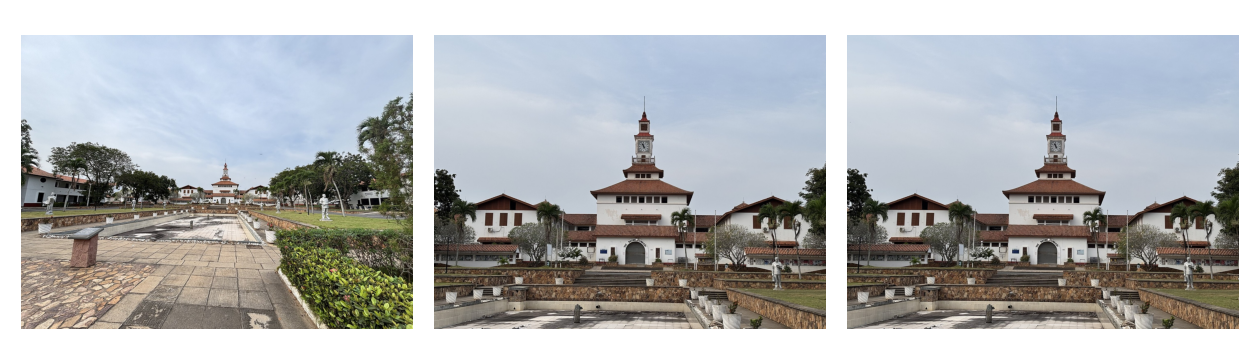
\includegraphics[width=0.98\linewidth]{figures/input_scene_main.png}
\caption{Three Balme Library views from \texttt{scene\_main}, the primary stitch set.}
\label{fig:input}
\end{figure*}

\section{Implementation}

The pipeline is shared by the batch experiments and the Streamlit walkthrough.

\begin{table}[t]
\centering
\setlength{\tabcolsep}{2.8pt}
{\small
\begin{tabular}{|l|p{0.48\linewidth}|}
\hline
Module & Responsibility \\
\hline\hline
\texttt{preprocess.py} & Resize, denoise, CLAHE \\
\texttt{features.py} & SIFT and ORB \\
\texttt{matching.py} & $k$NN and Lowe ratio \\
\texttt{homography.py} & RANSAC, composition, warp \\
\texttt{stitch.py} & Canvas and feather blend \\
\texttt{pipeline.py} & Pair matching and multi-image stitch \\
\texttt{evaluate.py} & Inlier ratio, reprojection, SSIM \\
\texttt{robustness.py} & Rotate, scale, brightness \\
\texttt{run\_experiments.py} & Tables and figures \\
\texttt{streamlit\_app.py} & Interactive walkthrough \\
\hline
\end{tabular}
}
\caption{Code layout under \texttt{src/} and \texttt{scripts/}.}
\label{tab:code}
\end{table}

\section{Experimental Results}

\subsection{Detector comparison}

Numbers in Table~\ref{tab:det} are from \texttt{report/results/detector\_comparison.csv} on consecutive Balme Library pairs. Full three-image stitch: SIFT $0.78$\,s, ORB $0.85$\,s. Mean inlier ratios are high (SIFT $0.951$, ORB $0.909$). Pair 2--3 is a near-duplicate facade (SSIM $0.976$, SIFT reprojection $0.23$\,px). Pair 1--2 maps the courtyard axis onto that facade and is the harder geometry (SSIM $0.76$, SIFT $1.38$\,px). Both panoramas are visually complete (Figure~\ref{fig:panos}).

\begin{table*}[t]
\centering
\setlength{\tabcolsep}{2.6pt}
{\scriptsize
\begin{tabular}{|l|c|c|c|c|c|c|c|c|}
\hline
Det. & Pair & Kpts (L/R) & Init.\ matches & Inliers & Ratio & Reproj.\ (px) & SSIM & Time (s) \\
\hline\hline
SIFT & 1--2 & 2000 / 2001 & 87 & 80 & 0.920 & 1.381 & 0.762 & 0.095 \\
SIFT & 2--3 & 2001 / 2000 & 1451 & 1426 & 0.983 & 0.225 & 0.976 & 0.068 \\
ORB & 1--2 & 2000 / 2000 & 34 & 28 & 0.824 & 2.152 & 0.712 & 0.115 \\
ORB & 2--3 & 2000 / 2000 & 1490 & 1481 & 0.994 & 0.794 & 0.975 & 0.039 \\
\hline
\end{tabular}
}
\caption{SIFT versus ORB on consecutive pairs of \texttt{scene\_main} (Balme Library). Inlier ratio is inliers over initial matches after Lowe's test. Reprojection is the mean error of RANSAC inliers.}
\label{tab:det}
\end{table*}

\begin{figure}[t]
\centering
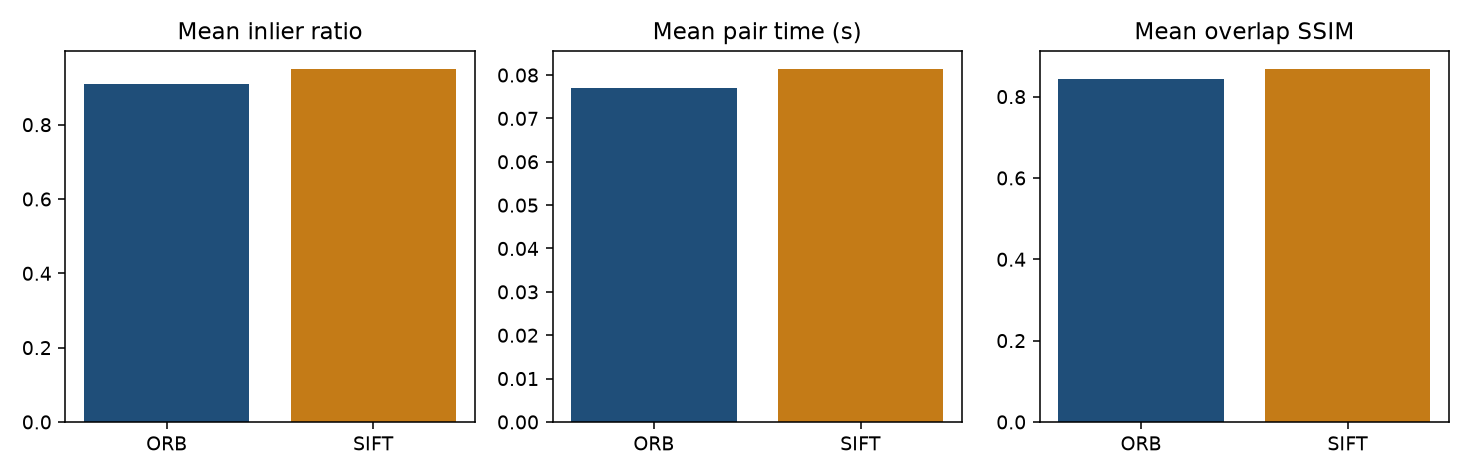
\includegraphics[width=0.98\linewidth]{figures/detector_comparison.png}
\caption{Summary of keypoint count, inlier ratio, reprojection error, and pair time for SIFT versus ORB.}
\label{fig:detplot}
\end{figure}

\begin{figure*}[t]
\centering
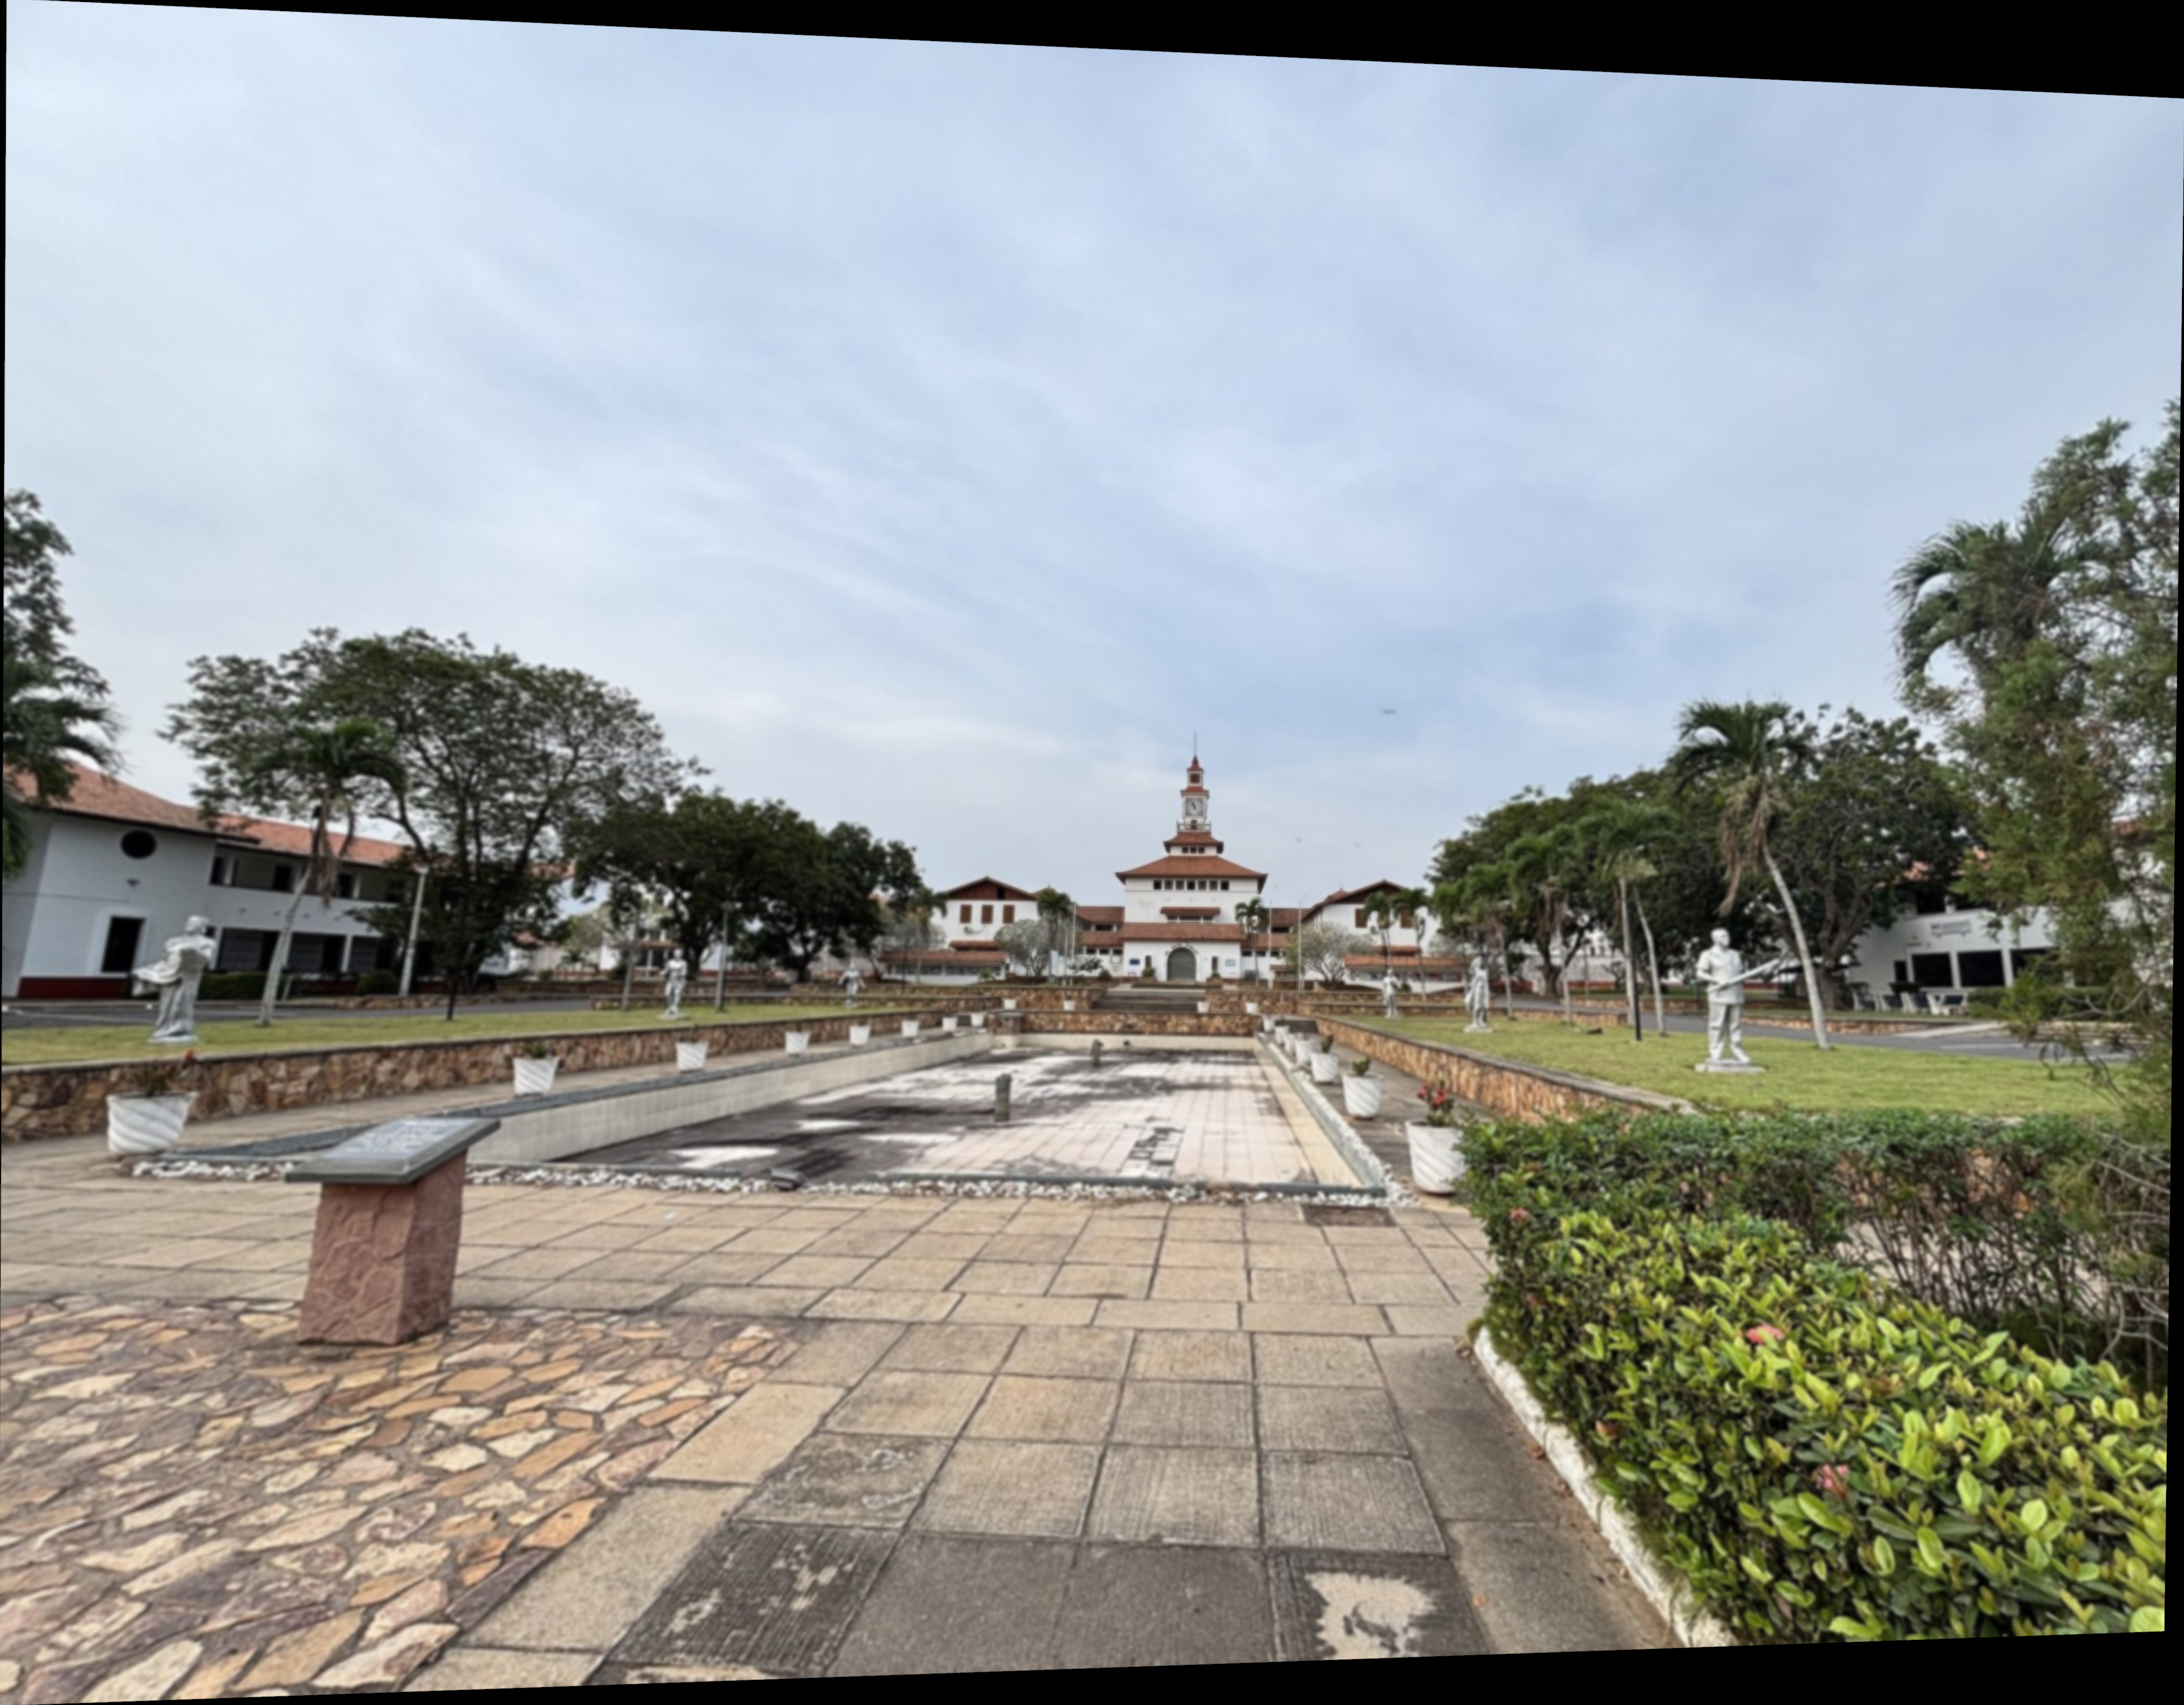
\includegraphics[width=0.48\linewidth]{figures/panorama_sift.png}\hfill
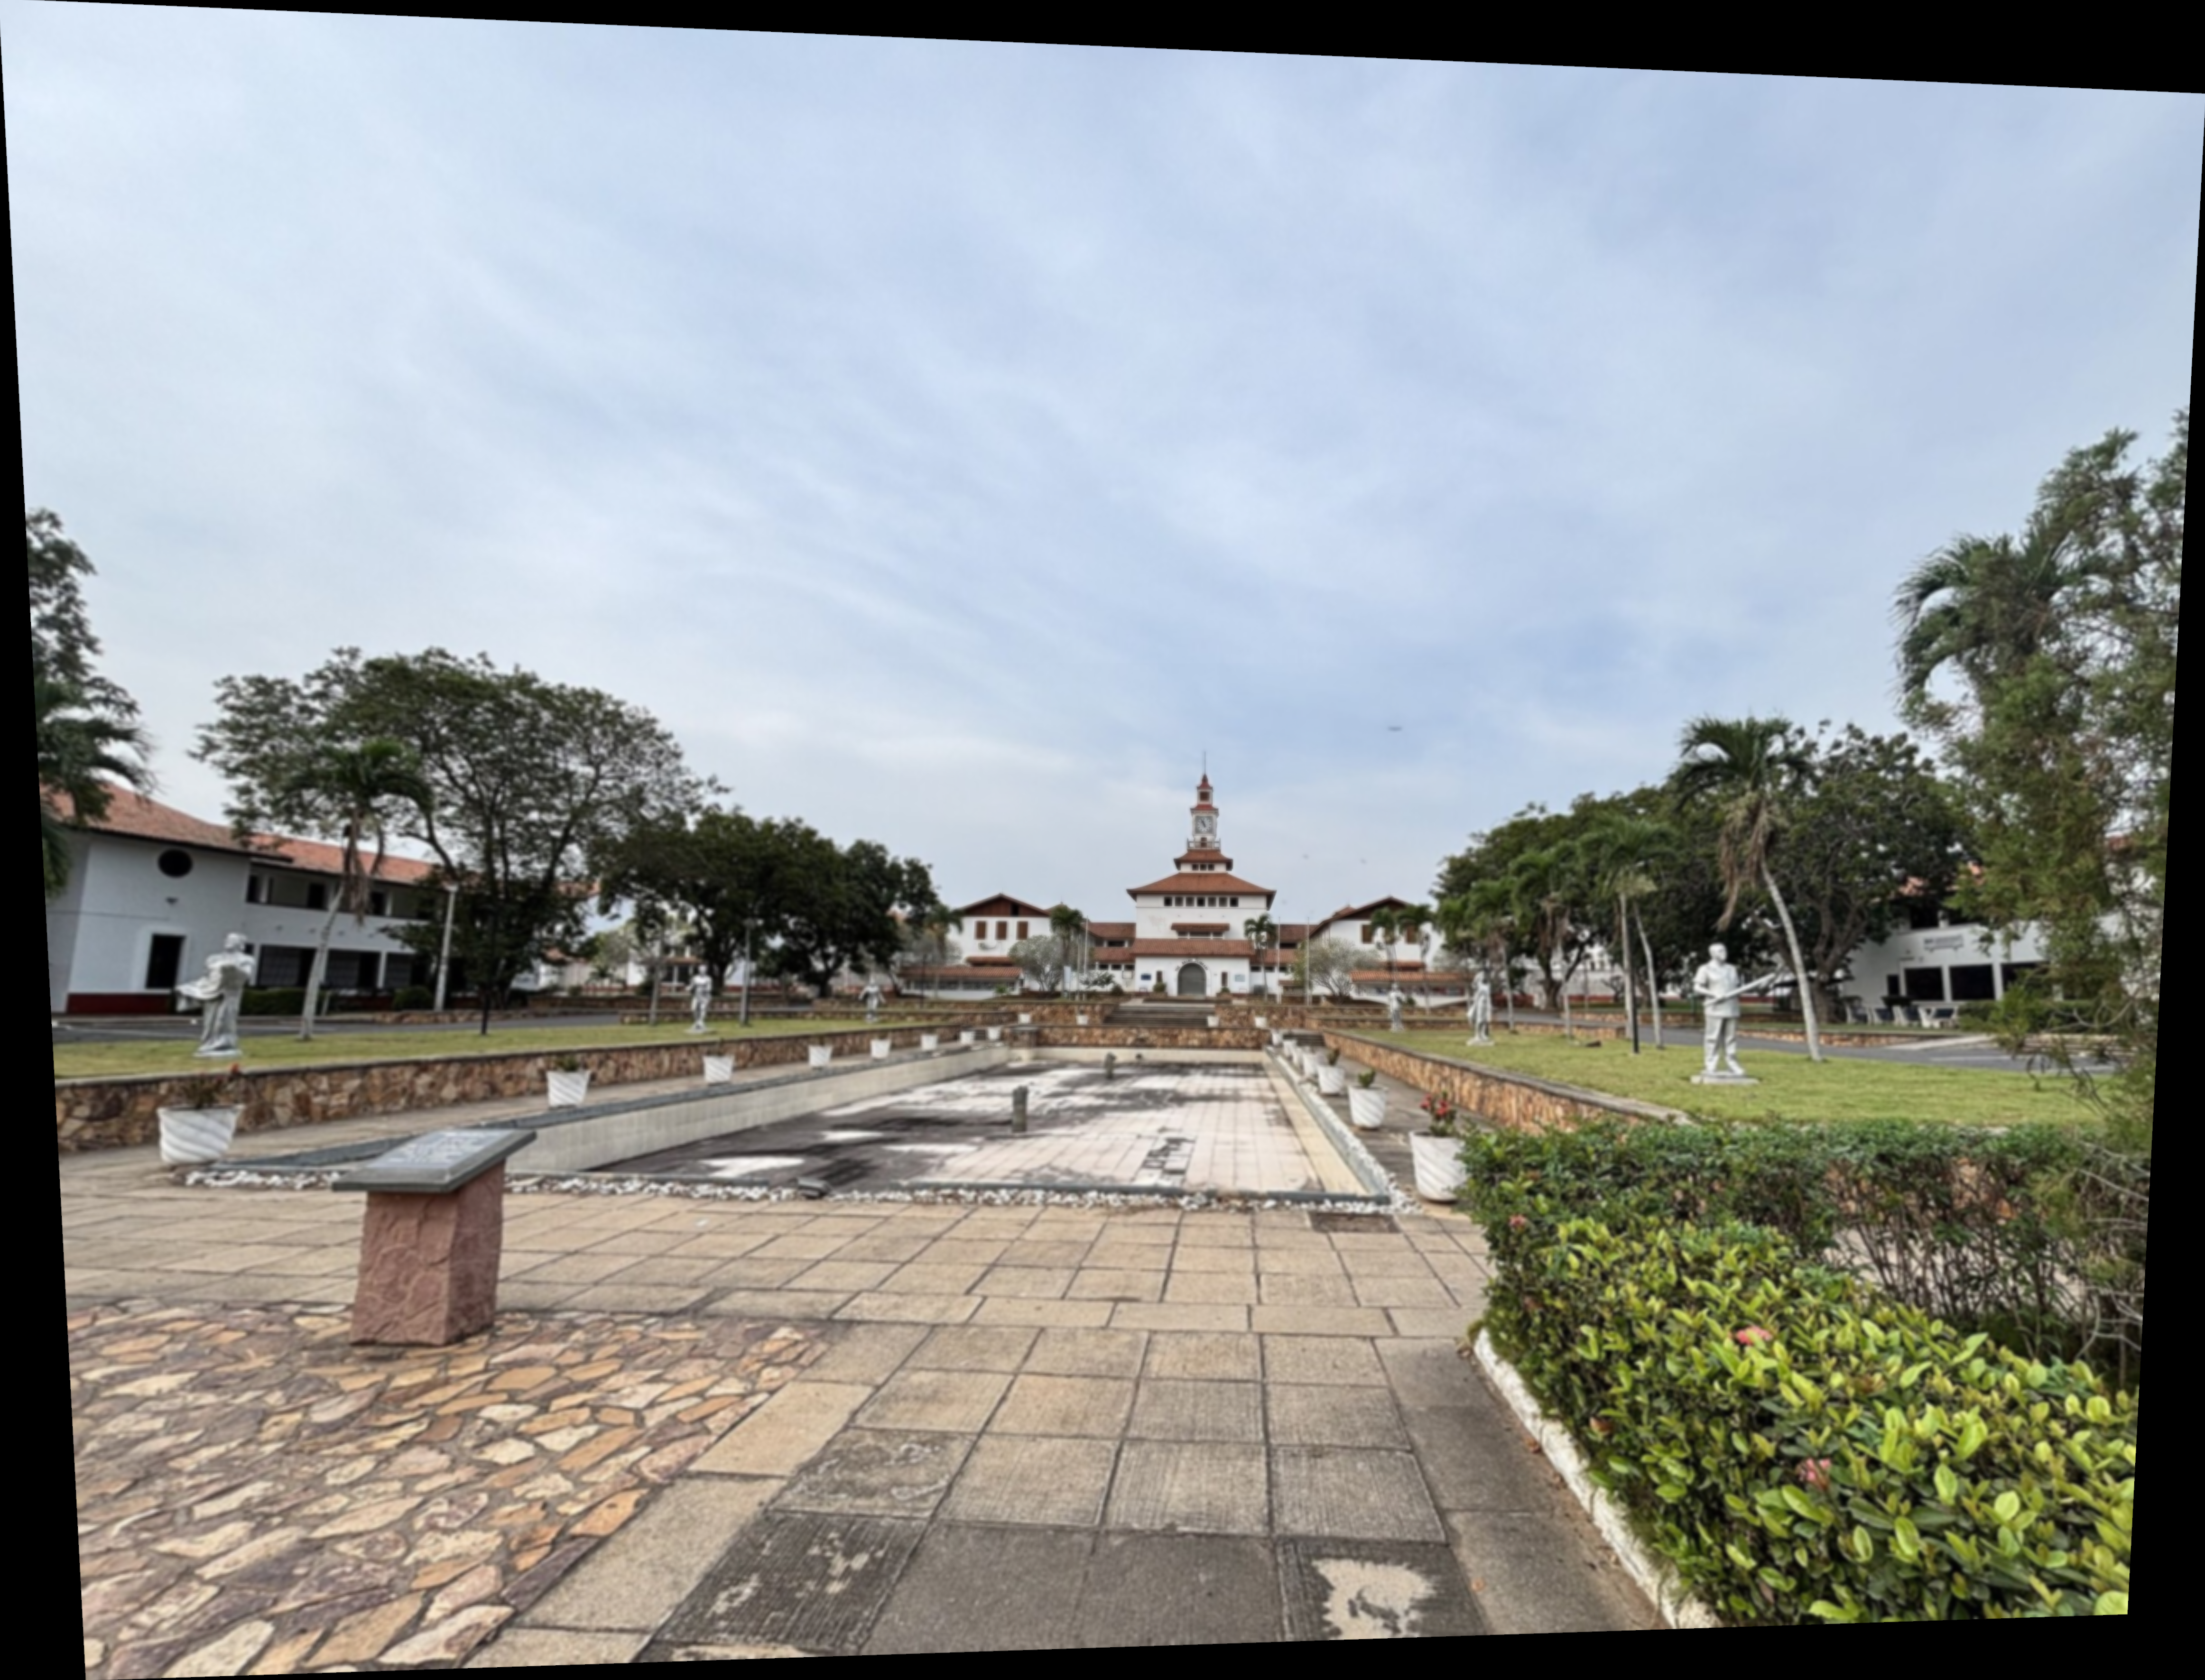
\includegraphics[width=0.48\linewidth]{figures/panorama_orb.png}
\caption{Three-image panoramas of Balme Library. Left: SIFT. Right: ORB. Both stitches are complete; pair 2--3 is a near-duplicate facade.}
\label{fig:panos}
\end{figure*}

\subsection{Robustness}

\paragraph{Rotation.}
On the courtyard-to-facade pair, inlier ratio stays high across $15^\circ$--$90^\circ$ (SIFT about $0.87$--$0.92$). The library has many distinctive windows and roof tiles, so a right-angle rotation is still matchable. SIFT's reprojection stays around $1.1$--$1.5$\,px; ORB sits near $2$\,px.

\paragraph{Scale.}
Half-size still works on this pair (SIFT 93 inliers, ratio $0.92$). At $1.5\times$ SIFT's ratio dips to $0.85$. The facade is feature-rich enough that moderate scale change is not the breaking case.

\paragraph{Illumination.}
A modest darkening (gain $0.55$) remains usable (SIFT ratio $0.86$). At gain $0.35$ SIFT finds no inliers; ORB reports 4, which is not a trustworthy homography. Brightening (gain $1.45$) hurts ORB more (ratio $0.59$ versus SIFT $0.80$). Neighbouring Night Market stalls (the lighting-folder pair) keep inlier ratios around $0.72$--$0.77$.

\paragraph{Viewpoint.}
Dance Department street versus courtyard or side views drop overlap SSIM to about $0.17$--$0.28$ and leave only a handful of inliers (ORB finds none on front--side). That is where the homography model has almost nothing to work with: the photographer moved around the building instead of rotating in place.

\begin{figure*}[t]
\centering
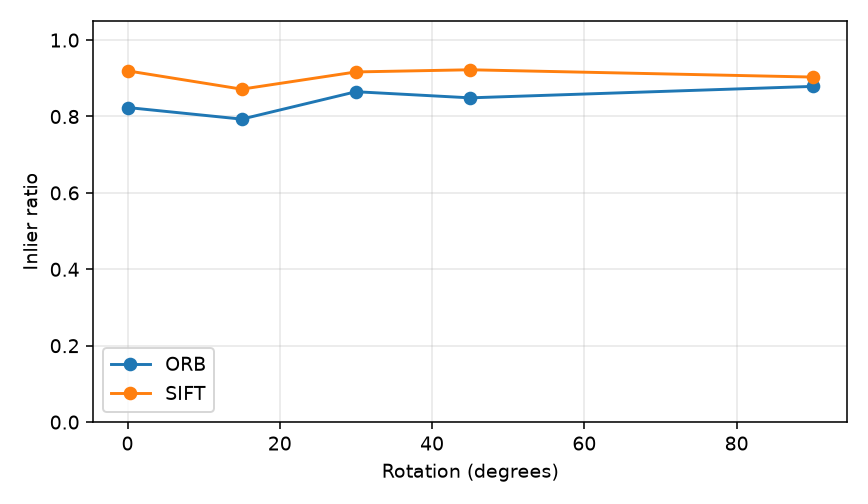
\includegraphics[width=0.48\linewidth]{figures/robustness_rotation.png}\hfill
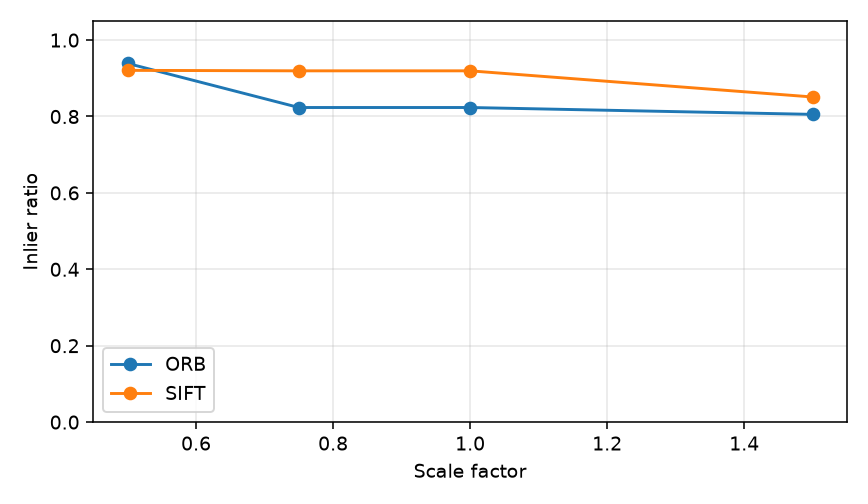
\includegraphics[width=0.48\linewidth]{figures/robustness_scale.png}\\[0.4em]
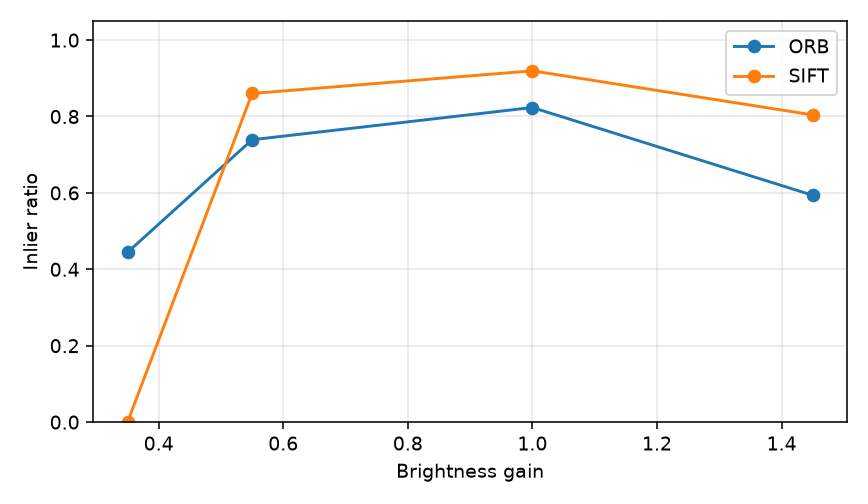
\includegraphics[width=0.48\linewidth]{figures/robustness_illumination.png}\hfill
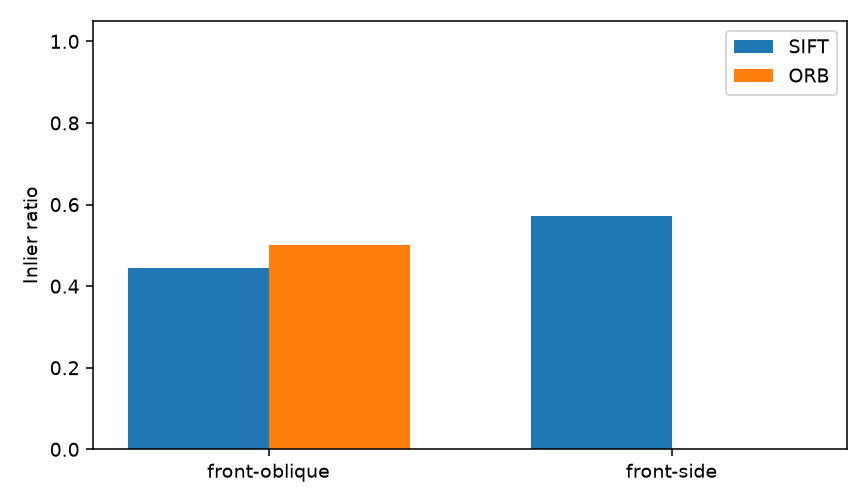
\includegraphics[width=0.48\linewidth]{figures/robustness_viewpoint.png}
\caption{Robustness sweeps. Top left: rotation. Top right: scale. Bottom left: illumination gain (and a dedicated lighting pair). Bottom right: viewpoint change off the plane.}
\label{fig:robust}
\end{figure*}

\subsection{Quantitative summary}

\begin{itemize}
\item \textbf{Keypoints} --- both detectors hit the 2000 cap on Balme Library.
\item \textbf{Initial matches} --- pair 2--3 returns over 1400 Lowe survivors; pair 1--2 is much thinner (SIFT 87, ORB 34).
\item \textbf{RANSAC inliers / inlier ratio} --- high on the library facade; SIFT contributes more inliers on the courtyard pair.
\item \textbf{Processing time} --- ORB is faster on pair 2--3 (binary matching); full-stitch times are close.
\item \textbf{Panorama quality} --- overlay SSIM $0.98$ on the near-duplicate facade and $0.76$ on courtyard-to-facade; mean reprojection error still favours SIFT.
\end{itemize}

\begin{figure*}[t]
\centering
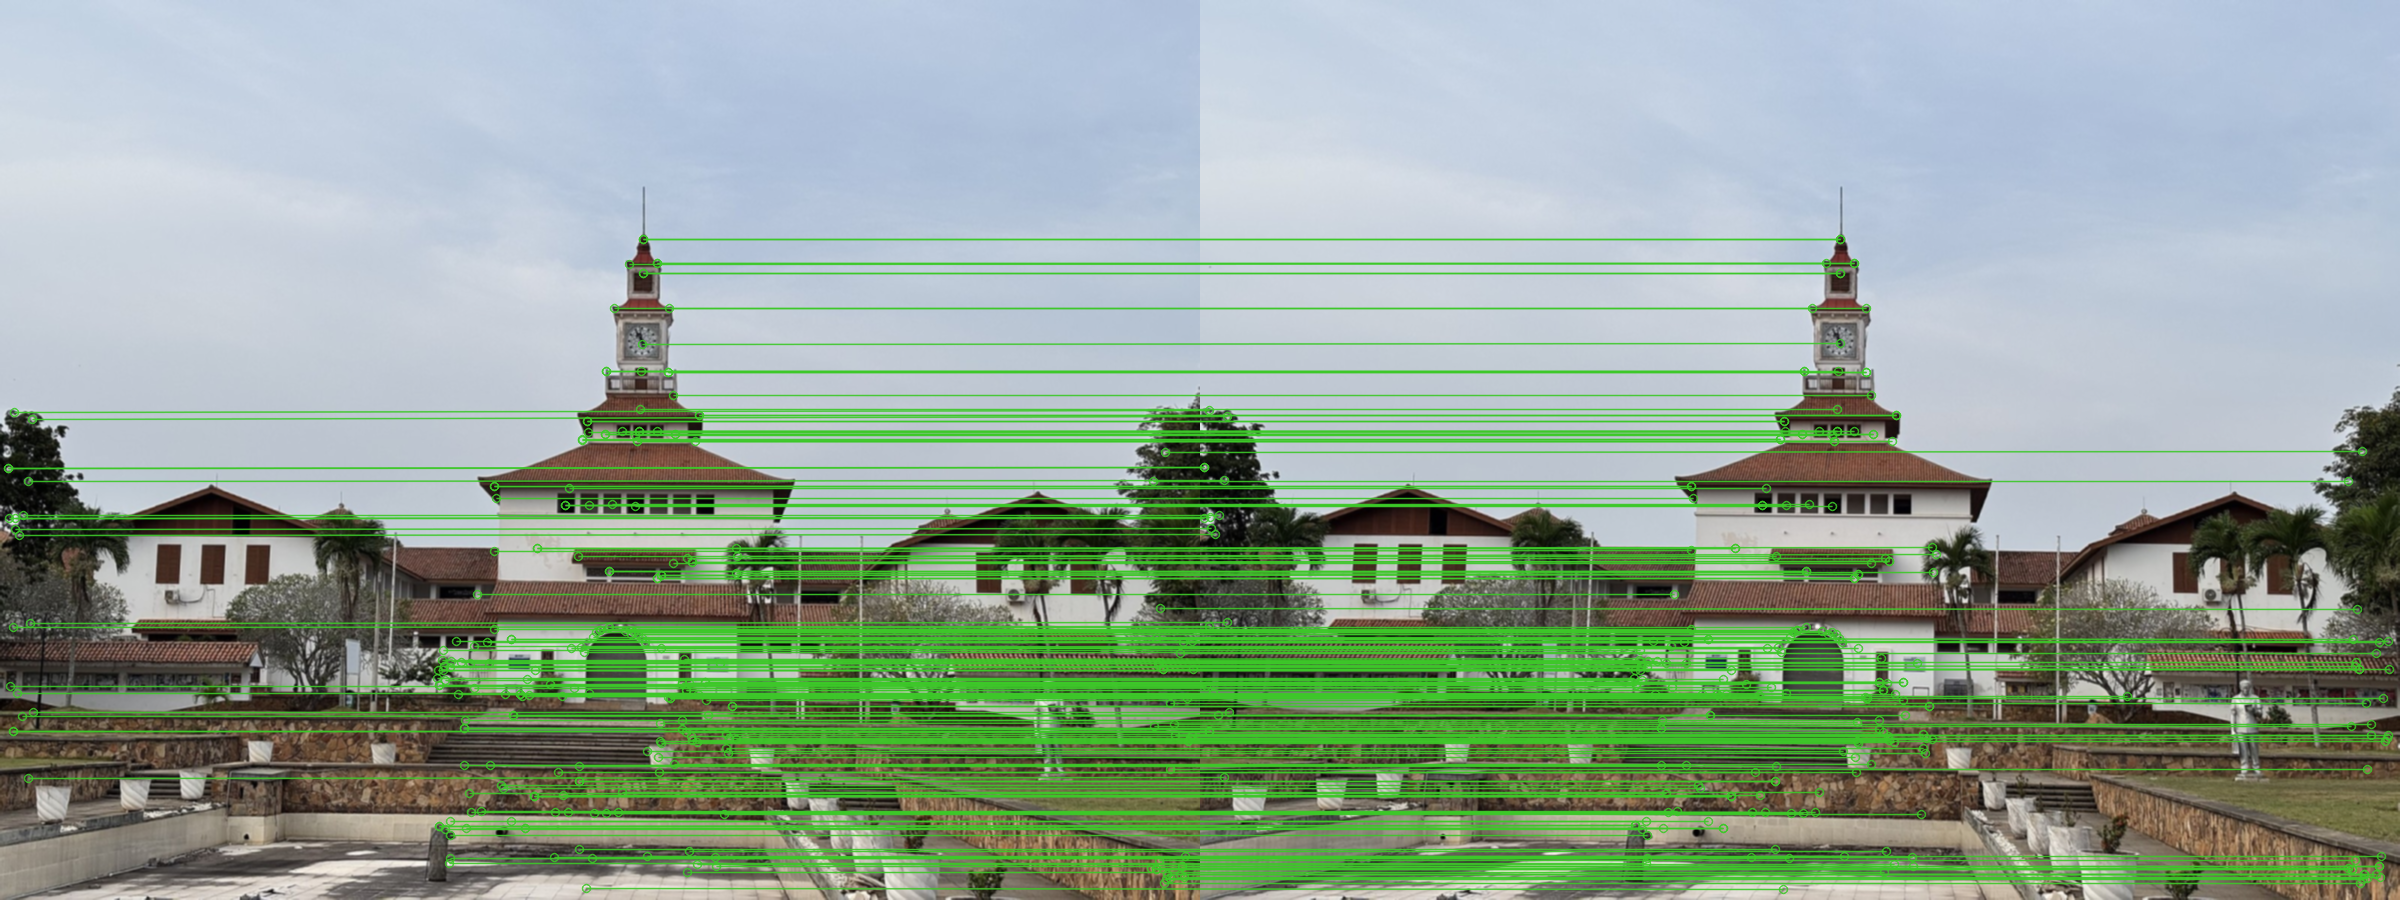
\includegraphics[width=0.48\linewidth]{figures/matches_after_sift.png}\hfill
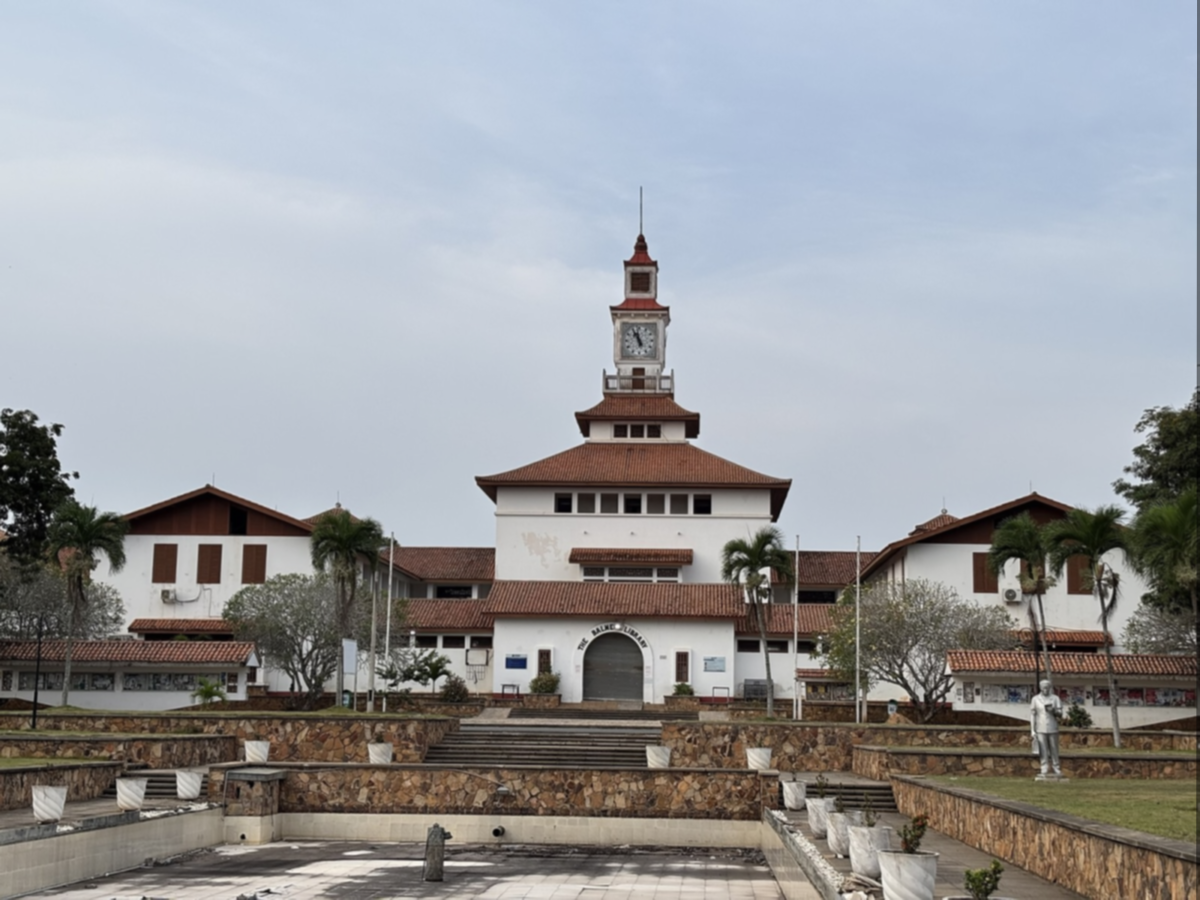
\includegraphics[width=0.48\linewidth]{figures/warp_overlay_sift.png}
\caption{Left: SIFT inliers after RANSAC on a main pair. Right: warped overlay of the same pair. The Streamlit application shows keypoints, putative matches, inliers, the overlay, and the final panorama interactively.}
\label{fig:matches}
\end{figure*}

\section{Discussion and Limitations}

\begin{enumerate}
\item \textbf{Homography assumes a plane (or pure rotation).} Trees, people, or a nearby object with parallax will ghost. The Dance Department viewpoint set already leaves too few inliers for a stable model.
\item \textbf{Low overlap.} Commons walk-up sequences (Commonwealth Hall) and unrelated building angles (Dance Department) are not a dedicated panorama capture. Below a handful of consistent inliers, RANSAC may still return a matrix that is geometrically meaningless.
\item \textbf{Severe illumination.} Gain $0.35$ leaves SIFT with zero inliers on the courtyard pair.
\item \textbf{Moving objects} in the Night Market overlap would generate persistent outliers; RANSAC can ignore some of them, but the blend will still ghost.
\item \textbf{Public photo sets.} Wikimedia frames are real Legon photographs with proper licences, but they were not shot for stitching. A phone capture with 30--50\% overlap from one spot would be a cleaner test.
\item \textbf{Near-duplicate frames.} Balme Library 2 and 3 are almost the same facade, so pair 2--3 overstates how easy a true multi-view stitch is.
\item \textbf{Feather blending} cannot hide large exposure differences or parallax; a multi-band blend would be a natural extension.
\item \textbf{Feature budget.} Capping at 2000 keypoints is a speed choice; a textureless wall would need a different detector response threshold, not a higher cap.
\end{enumerate}

\section{Conclusion}

The system demonstrates the full classical chain from overlapping views to a panorama, with SIFT and ORB compared on the metrics listed above. On Balme Library photographs both detectors stitch a complete three-image panorama; SIFT is the more accurate geometric estimator on the courtyard pair, the close facade pair is easy for both, and both break when the light is crushed or the viewpoint leaves the overlapping region. The interactive application makes each of those statements visible without treating stitching as a black box.

{\small
\bibliographystyle{ieee}
\bibliography{references}
}

\end{document}
